\documentclass[border=9pt]{standalone}
\usepackage[fontset=fandol]{ctex}
\usepackage{amsmath,amssymb,tikz}
\usetikzlibrary{arrows.meta,calc,decorations.pathmorphing}
\tikzset{arr/.style={-{Stealth[length=2mm]},semithick}}
\begin{document}

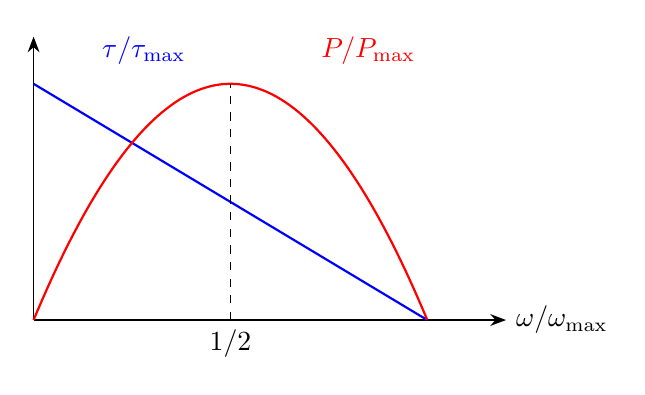
\begin{tikzpicture}[xscale=5,yscale=3]
\draw[arr] (0,0)--(1.2,0) node[right] {$\omega/\omega_{\max}$};
\draw[arr] (0,0)--(0,1.2);
\draw[thick,blue] (0,1)--(1,0);
\draw[thick,red,domain=0:1,samples=90] plot(\x,{4*\x*(1-\x)});
\node[blue] at (.28,1.14) {$\tau/\tau_{\max}$};
\node[red] at (.85,1.14) {$P/P_{\max}$};
\draw[dashed] (.5,0)--(.5,1);\node[below] at (.5,0) {$1/2$};
\end{tikzpicture}

\end{document}
